\documentclass[letterpaper]{article}
\title{16831 Statistical Techniques, Fall 2011\\Homework 5: Online Learning}
\date{December 7th, 2011}
\author{Natasha Kholgade and Marynel V\'azquez}
\usepackage[margin=1in]{geometry}
\usepackage{amsmath}
\usepackage{amssymb}
\usepackage{url}
\usepackage{graphicx}
\usepackage{color}
% Make URL click-able
\usepackage{hyperref}

% Don't indent after paragraphs
\parindent 0in
\parskip 4pt

\begin{document}

\maketitle

\section*{Classifiers}

For this homework, we implemented Gaussian Process Regression (GPR),
Adaptive Boosting, and online linear SVMs. We used these algorithms in a binary
fashion to classify 3D points into five different classes: Vegetation,
Wire, Pole, Ground and Facade. Each classifier was trained 5 times in
a one-vs-all scenario, such that the final classification for a
testing data point was given by the class with highest score.

GPR and boosting were not implemented in an online fashion (though
boosting does lend itself to an online implementation, we were limited
in time). Our version of Gaussian Process Regression uses the
exponential to the negative squared distance between features (radial
basis function) as the covariance function. Meanwhile, boosting
performs feature selection, and uses the exponentiated gradient as
suggested by Alex Grubb. We use thresholded decision stumps as linear
classifiers in boosting.

Our implementation of a Supper Vector Machine is based on the
subgradient of the hinge loss, plus a regularization term. It operates
fast, though requires a significant number of samples to satisfactory
classify new data in comparison to the other algorithms being
considered.

\section*{Performance Summary}

For this homework, we performed two-fold cross-validation on data from
one file, and then tested with data from the other file. We swapped
the two files, and re-did cross-validation and training. We provide
the best parameters, confusion matrices, per-class percentage
performance, and net classification rate for the three classes.

For brevity, we refer to the point cloud data file
\textit{oakland\_part3\_am\_rf.node\_features} as \textit{File\_am}, and
to the file \textit{oakland\_part3\_an\_rf.node\_features} as
\textit{File\_an} in the following sections.

\subsection*{Gaussian Process Regression}

\textbf{Train with \textit{File\_am}, and test with \textit{File\_an}:}

Best parameters: radial basis function parameter $\sigma=.4$,
regularization parameter $\lambda=.4642$.

Net classification rate: .8637

Per-class classification rate: 
$$\begin{bmatrix}0.8208   & 0.8870  &  0.7192   & 0.9796 &   0.6670\end{bmatrix}$$

Confusion matrix:
$$\begin{bmatrix}
0.8208 &   0.0560  & 0.0407 &   0.0015  &  0.0809\\
    0.0758&    0.8870 &   0.0084&    0.0004 &   0.0285\\
    0.1971   & 0.0092   & 0.7192  &  0.0046   & 0.0700\\
    0.0018   & 0.0179    &0.0003  &  0.9796  &  0.0005\\
    0.1316   &0.1576    &0.0421  &  0.0017  &  0.6670
\end{bmatrix}$$

\textbf{Train with \textit{File\_an}, and test with \textit{File\_am}:}

Best parameters: radial basis function parameter $\sigma=.4$, regularization parameter $\lambda=.4642$.

Net classification rate: .947

Per-class classification rate: 
$$\begin{bmatrix}0.8097  &  0.5697   & 0.9279   & 0.9899  &  0.8305\end{bmatrix}$$

Confusion matrix:
$$\begin{bmatrix}
0.8097&    0.0471&    0.0680  &  0.0010  &  0.0743\\
    0.0685&    0.5697&    0.0183&    0.0697  &  0.2738\\
    0.0378   & 0.0014&    0.9279  &       0 &   0.0329\\
    0.0020 &   0.0001 &   0.0065 &   0.9899  &  0.0014\\
    0.0611   & 0.0391  &  0.0686  &  0.0007&    0.8305\\
\end{bmatrix}$$


\subsection*{Linear SVMs}

\subsection*{AdaBoost}

\textbf{Train with \textit{File\_am}, and test with \textit{File\_an}:}

Best parameters: Running time $T=140$, gradient projection threshold $\eta=1e-4$.

Net classification rate: .8663

Per-class classification rate: 
$$\begin{bmatrix} 0.8403  &  0.8560   & 0.7017 &   0.9798  &  0.6476\end{bmatrix}$$

Confusion matrix:
$$\begin{bmatrix}
    0.8403 &   0.0381  &  0.0437  &  0.0013  &  0.0765\\
    0.0770  &  0.8560   & 0.0088   & 0.0193  &  0.0389\\
    0.1888  &  0.0120   & 0.7017   & 0.0055  &  0.0921\\
    0.0022  &  0.0160   & 0.0001   & 0.9798  &  0.0018\\
    0.1221  &  0.1457   & 0.0702   & 0.0145  &  0.6476
\end{bmatrix}$$

\textbf{Train with \textit{File\_an}, and test with \textit{File\_am}:}

Best parameters: Running time $T=140$, gradient projection threshold $\eta=1e-4$.

Net classification rate: .9495

Per-class classification rate: 
$$\begin{bmatrix}0.8178 &   0.6320 &   0.9104  &  0.9948  &  0.8148\end{bmatrix}$$

Confusion matrix:
$$\begin{bmatrix}
0.8178 &   0.0494   & 0.0656 &   0.0022  &  0.0650\\
    0.0477 &   0.6320  &  0.0244 &   0.0489 &   0.2469\\
    0.0378 &   0.0203 &   0.9104  &  0.0007  &  0.0308\\
    0.0031  &  0.0005 &   0.0010  &  0.9948  &  0.0007\\
    0.0547  &  0.0578   & 0.0724  &  0.0003  &  0.8148
\end{bmatrix}$$

\subsection*{Time}

AdaBoost takes on average a long time to train (148 seconds) but just 1.12 seconds in testing as we just apply a set of thresholded linear classifiers and take their sum. GPR takes lesser training time (12.19 seconds), but it takes a longer test time (26.83 seconds), because we apply the product of the training kernel matrix inverse and the training labels (which can be precomputed) to all the kernel vectors formed with every test point to all training points.

\subsection*{Misclassifications}
We find that points belonging to the `Pole', `Wire', and `Facade' classes do not always perform well because there is not enough data to train them.

\subsection*{Ease of Implementation}

GPR and SVM were relatively easy to implement. AdaBoost required a bit of delving into some math, but 
we made it through.

\subsection*{Robustness to noise}
GPR is robust to noise. When we added a whole bunch of noise to the features, we still get net classification rates of .865 and .94, and per-class correct classifications:
$$\begin{bmatrix} 0.8417 &   0.8614 &   0.7164   & 0.9806  &  0.6263\end{bmatrix}$$
$$\begin{bmatrix} 0.7809  &  0.5733  &  0.9440&    0.9969    &0.7608\end{bmatrix}$$
Noise-corrupted versions of features when passed through GPR are classified with rates .85 and .94, and per-class classifications are:
$$\begin{bmatrix} 0.8204  &  0.8757 &   0.6980  &  0.9796 &   0.5859\end{bmatrix}$$
$$\begin{bmatrix} 0.7779  &  0.5880  &  0.9286  &  0.9950 &   0.7704\end{bmatrix}$$

The same robustness is observed with AdaBoost. On adding a whole bunch of noise to the features, we get rates of .862, and .947, and per-class classifications of:
$$\begin{bmatrix} 0.8334 &   0.8514 &   0.6796  & 0.9775  &  0.6465\end{bmatrix}$$
$$\begin{bmatrix} 0.7985 &   0.6064   & 0.9146 &   0.9935 &   0.8167\end{bmatrix}$$
Noise-corrupted versions of features when passed through AdaBoost are classified with rates .8676 and .945, and per-class classifications are:
$$\begin{bmatrix} 0.8543 &   0.8548 &   0.6888&    0.9725  &  0.6410\end{bmatrix}$$
$$\begin{bmatrix} 0.8063  &  0.6112 &   0.9174  &  0.9918  &  0.8062\end{bmatrix}$$

We would most probably use AdaBoost for the robot because it is faster than Gaussian Process Regression during testing (though it performs just as well), and it performs better than the linear SVM. If we needed an online version of the training algorithm, we would probably use SVMs, but with kernels. We did not have time to implement the kernel SVMs, but we do notice that the dataset has some non-linearity as is evidenced by the better performance of GPR and AdaBoost.

\subsection*{Pictorial Result}
With GPR training with \textit{File\_am}, and testing with \textit{File\_an} gave us the scatter plot shown in \ref{Fig_GPR1}, while training with \textit{File\_an}, and testing with \textit{File\_am} gave us the plot in \ref{Fig_GPR2}
\begin{figure}
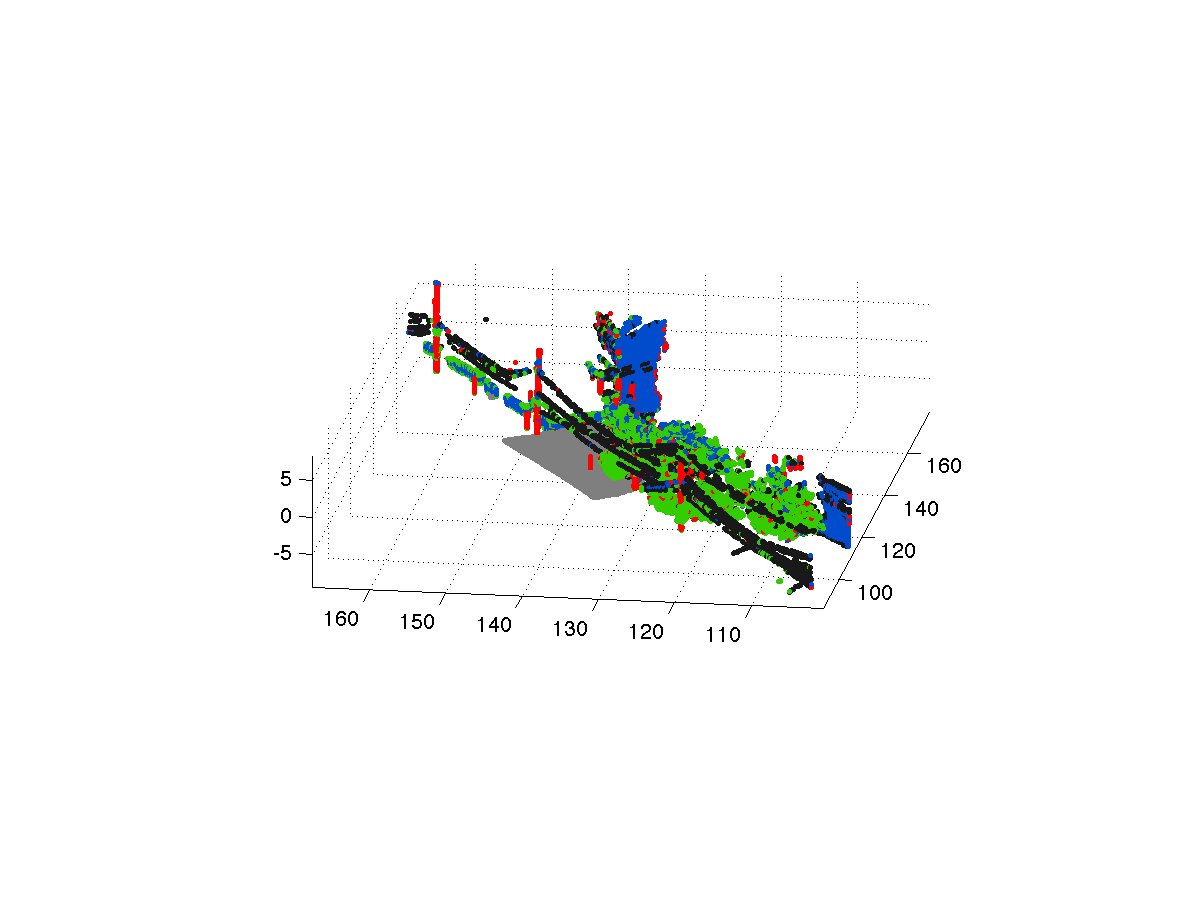
\includegraphics[width=\linewidth]{gpr_trainam_testan.png}
\caption{Scatter plot of points from File-am classified with GPR: green = vegetation, blue = facade, really dark gray = wire, red = pole, light gray = ground}
\label{Fig_GPR1}
\end{figure}
\begin{figure}
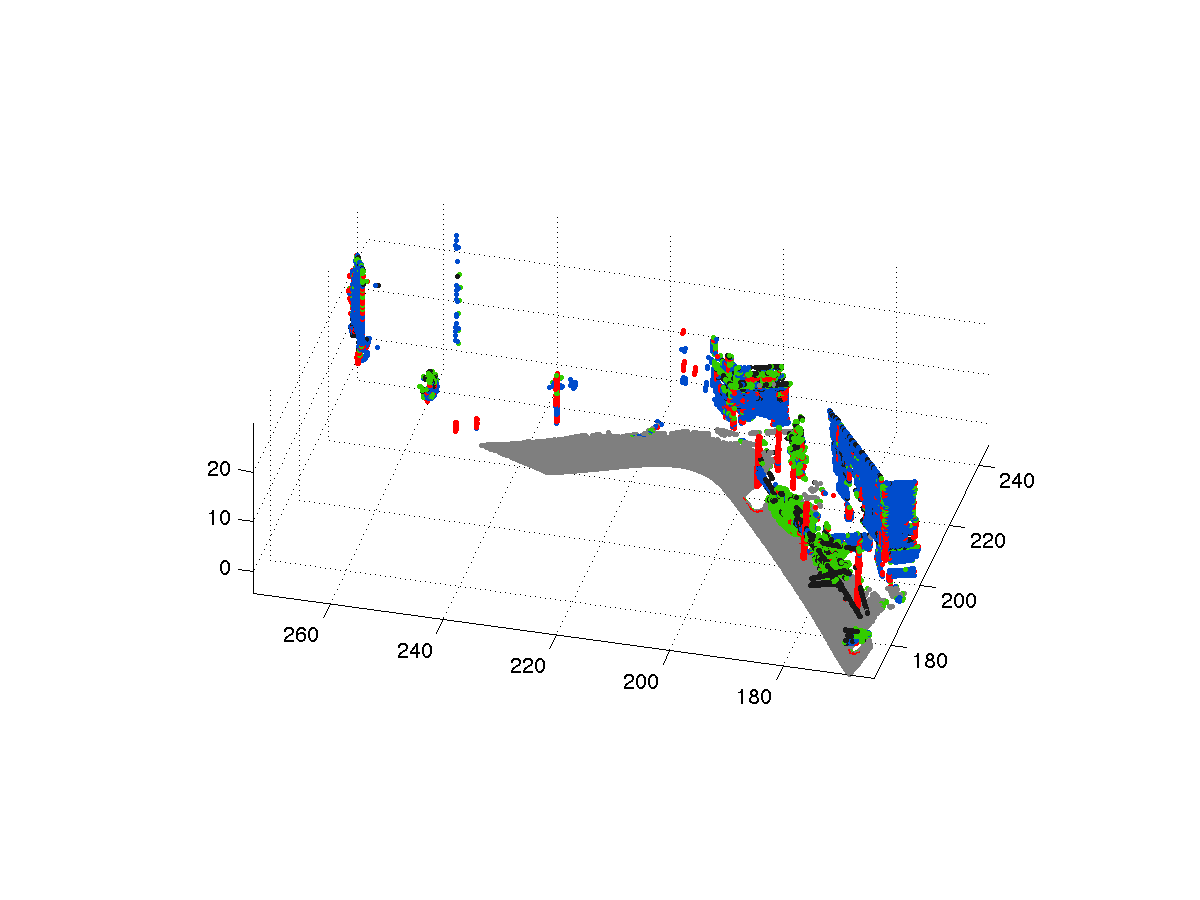
\includegraphics[width=\linewidth]{gpr_trainan_testam.png}
\caption{Scatter plot of points from File-an classified with GPR: green = vegetation, blue = facade, really dark gray = wire, red = pole, light gray = ground}
\label{Fig_GPR2}
\end{figure}

With AdaBoost training with \textit{File\_am}, and testing with \textit{File\_an} gave us the scatter plot shown in \ref{Fig_Ada1}, while training with \textit{File\_an}, and testing with \textit{File\_am} gave us the plot in \ref{Fig_Ada2}
\begin{figure}[t]
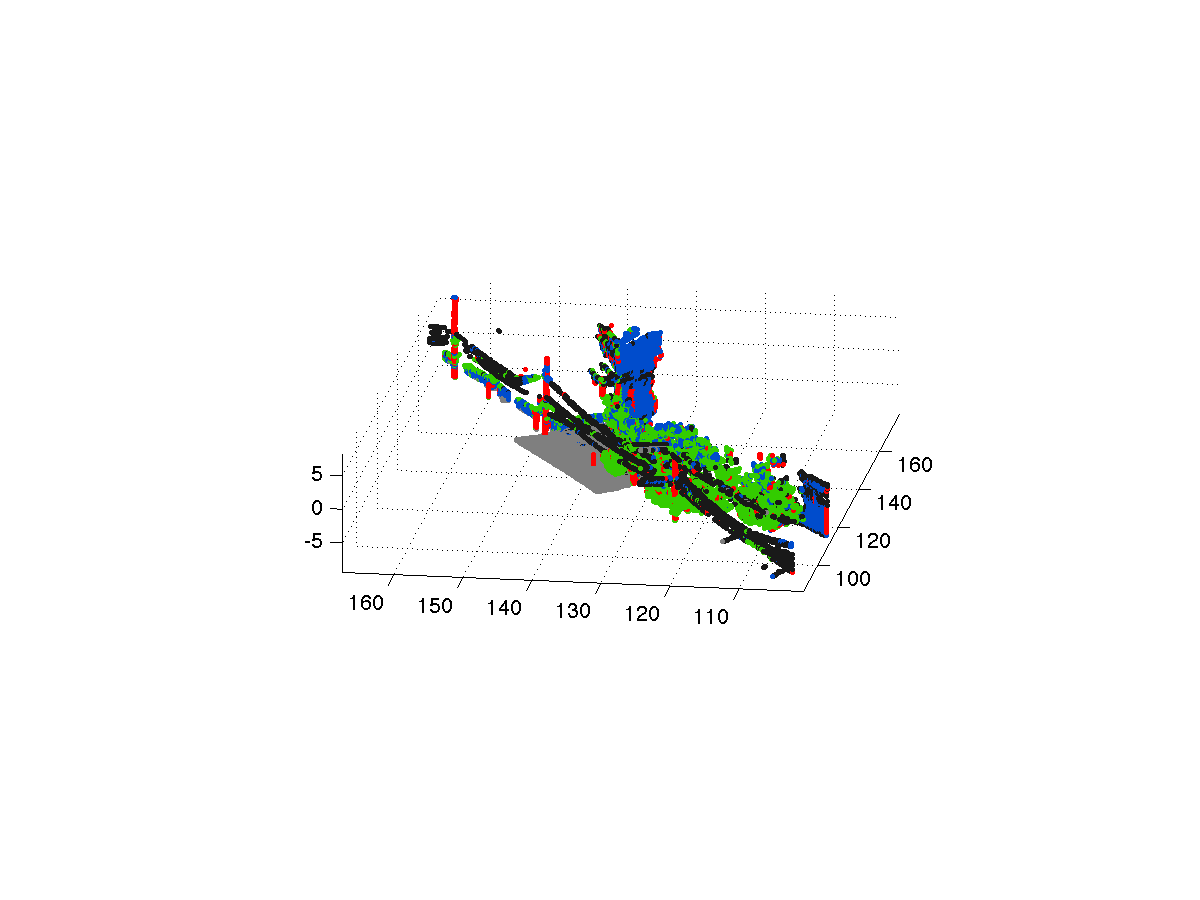
\includegraphics[width=\linewidth]{boost_trainam_testan.png}
\caption{Scatter plot of points from File-am classified with AdaBoost: green = vegetation, blue = facade, really dark gray = wire, red = pole, light gray = ground}
\label{Fig_Ada1}
\end{figure}
\begin{figure}
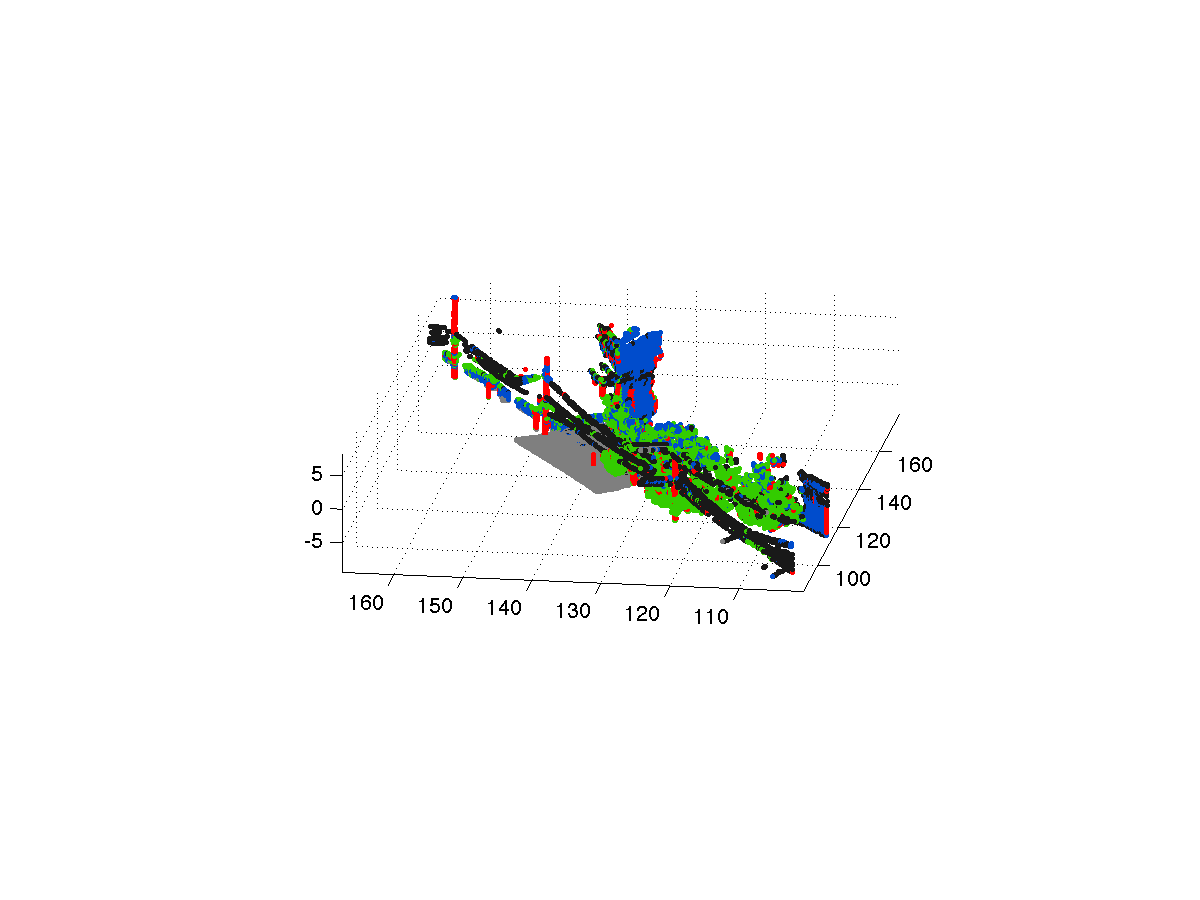
\includegraphics[width=\linewidth]{boost_trainam_testan.png}
\caption{Scatter plot of points from File-an classified with AdaBoost: green = vegetation, blue = facade, really dark gray = wire, red = pole, light gray = ground}
\label{Fig_Ada2}
\end{figure}


\begin{enumerate}
\item How well did it perform for online learning?  Does it perform well on the held-out data?
\item Are there any classes that did not get classified well?  Why do you think that is?
\item How easy was the learner to implement?
\item How long does the learner take (in terms of data points, dimensions, classes, etc...) for training and prediction?
\item Show images/movies of the classified data.  Note that MATLAB is not very good at displaying thousands of 3D points; use VRML or python.
\item How did you choose (hyper)parameters (priors, kernel width, noise variance, prior variance, learning rate, etc\ldots)?
\item How robust is this algorithm to noise? Take the current feature set and:
  \begin{itemize}
  \item Add a large number of random features
  \item Add a large number of features that are noise corrupted versions of the features already in the data-set.
  \end{itemize}

\end{enumerate}

You should also compare the learners' performance to each other.  Did kernels help on this data set?  Which one would you use on your robot?  What would future work include?

\end{document}
